% -----------------------------------------------------------------------------

\begin{frame}{Mother-child dyads}
    \begin{columns}[c] % The "c" option specifies centered vertical alignment while the "t" option is used for top vertical alignment

        \column{.6\textwidth} % Right column and width
    
        \begin{figure}
        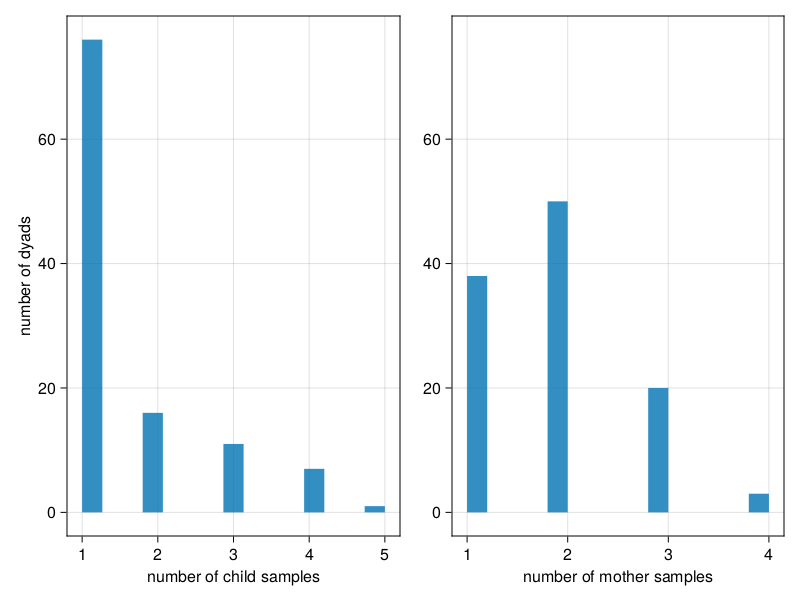
\includegraphics[width=1\linewidth]{../figures/dyads}
        \end{figure}

        \column{.4\textwidth} % Right column and width
    
        \textbf{Details}
        \begin{itemize}
            \item \textbf{Left} - Child samples that have at least 1 associated maternal sample
            \item \textbf{Right} - Maternal samples that have at least 1 associated child sample
        \end{itemize}

    \end{columns}

\end{frame}

% -----------------------------------------------------------------------------

\begin{frame}{Sample collection by age}
    \begin{columns}[c] % The "c" option specifies centered vertical alignment while the "t" option is used for top vertical alignment

        \column{.6\textwidth} % Right column and width
    
        \begin{figure}
        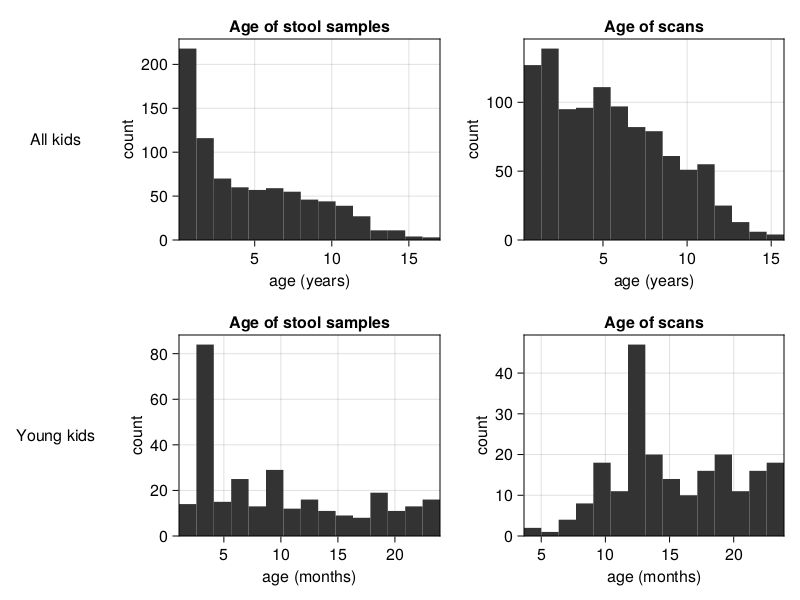
\includegraphics[width=1\linewidth]{../figures/age_hists}
        \end{figure}

        \column{.4\textwidth} % Right column and width
    
        \textbf{Details}
        \begin{itemize}
            \item Bottom row is same as top, but only from timepoints $<$ 24 months
        \end{itemize}

    \end{columns}

\end{frame}

% -----------------------------------------------------------------------------

\begin{frame}{Sample collection over time}
    \begin{columns}[c] % The "c" option specifies centered vertical alignment while the "t" option is used for top vertical alignment

        \column{.6\textwidth} % Right column and width
    
        \begin{figure}
        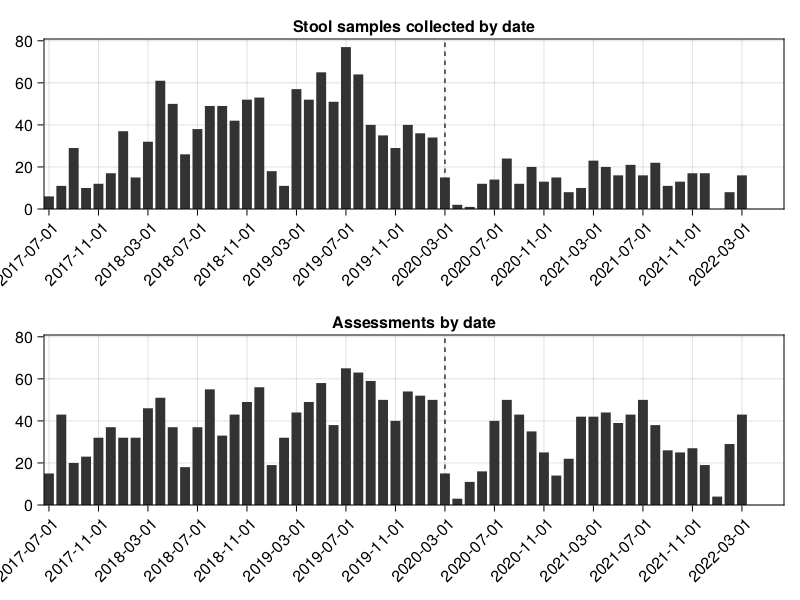
\includegraphics[width=1\linewidth]{../figures/collection_over_time}
        \end{figure}

        \column{.4\textwidth} % Right column and width
    
        \textbf{Details}
        \begin{itemize}
            \item \textbf{Top} - Stool samples (just omni) collected by date
            \item \textbf{Bottom} - Assessments (clinical visits) by date
        \end{itemize}

    \end{columns}

\end{frame}

% -----------------------------------------------------------------------------

\begin{frame}{Upset - Brain scans + stool}
    \begin{columns}[c] % The "c" option specifies centered vertical alignment while the "t" option is used for top vertical alignment

        \column{.6\textwidth} % Right column and width
    
        \begin{figure}
        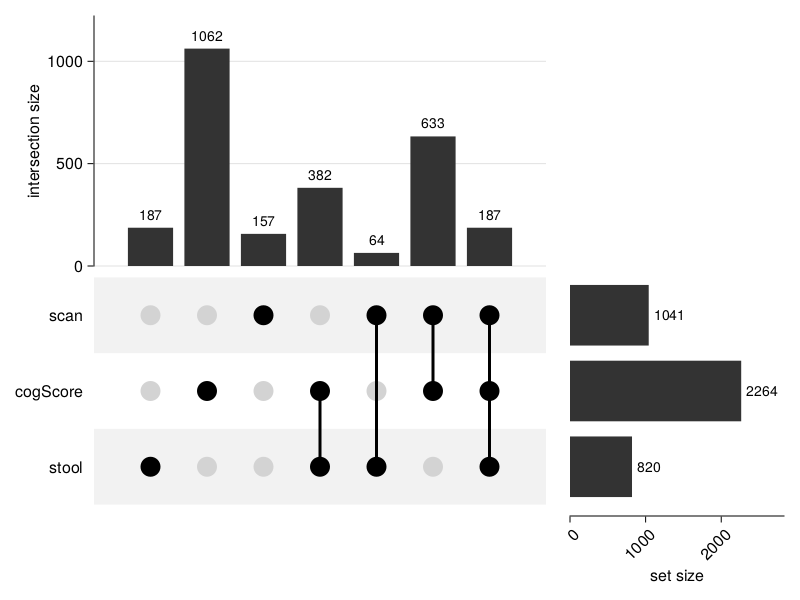
\includegraphics[width=1\linewidth]{../figures/upset_scan_stool.pdf}
        \end{figure}

        \column{.4\textwidth} % Right column and width
    
        \textbf{Details}
        \begin{itemize}
            \item Overlap of sample collection and brain scans
            \item "Prev stool" means that there's stool sample collected prior to timepoint
            \item Not 100\% sure of this code - needs review
        \end{itemize}

    \end{columns}

\end{frame}

% -----------------------------------------------------------------------------

\begin{frame}{Upset - By subject}
    \begin{columns}[c] % The "c" option specifies centered vertical alignment while the "t" option is used for top vertical alignment

        \column{.6\textwidth} % Right column and width
    
        \begin{figure}
        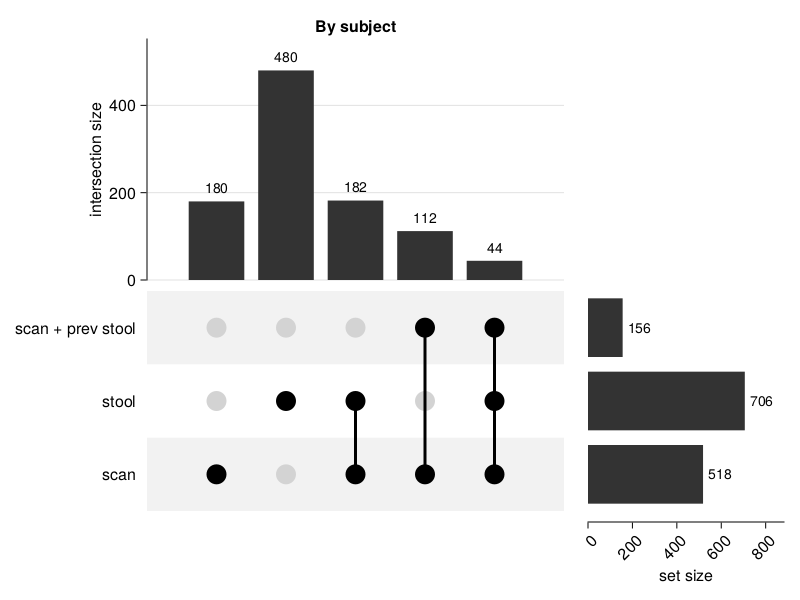
\includegraphics[width=1\linewidth]{../figures/upset_scan_stool_bysybject.pdf}
        \end{figure}

        \column{.4\textwidth} % Right column and width
    
        \textbf{Details}
        \begin{itemize}
            \item Overlap of sample collection and brain scans
            \item Numbers reduced to unique subjects
        \end{itemize}

    \end{columns}

\end{frame}

% -----------------------------------------------------------------------------

\begin{frame}{Upset - Overlaps with cogscore}
    \begin{columns}[c] % The "c" option specifies centered vertical alignment while the "t" option is used for top vertical alignment

        \column{.6\textwidth} % Right column and width
    
        \begin{figure}
        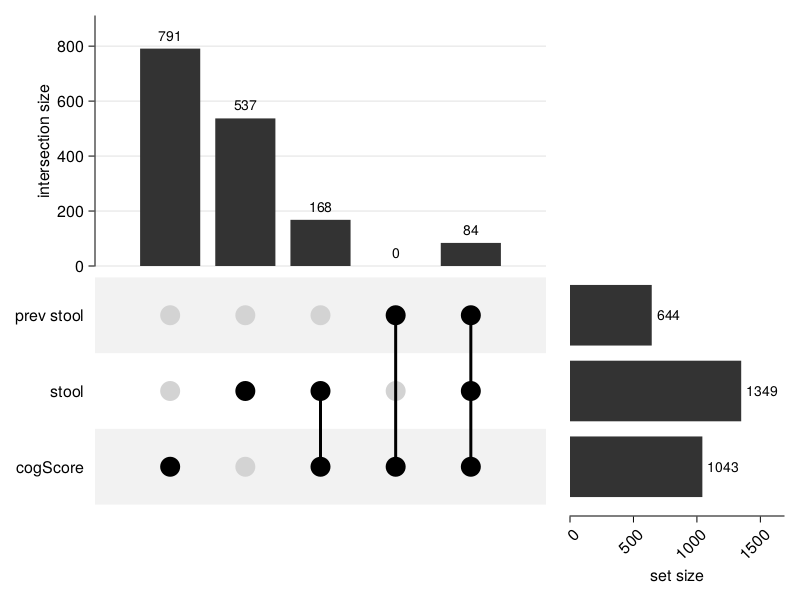
\includegraphics[width=1\linewidth]{../figures/upset_score_stool.pdf}
        \end{figure}

        \column{.4\textwidth} % Right column and width
    
        \textbf{Details}
        \begin{itemize}
            \item Overlap of sample collection and cognitive score
        \end{itemize}

    \end{columns}

\end{frame}

% -----------------------------------------------------------------------------
\begin{frame}{Upset - Kids under 3}
    \begin{columns}[c] % The "c" option specifies centered vertical alignment while the "t" option is used for top vertical alignment

        \column{.6\textwidth} % Right column and width
    
        \begin{figure}
        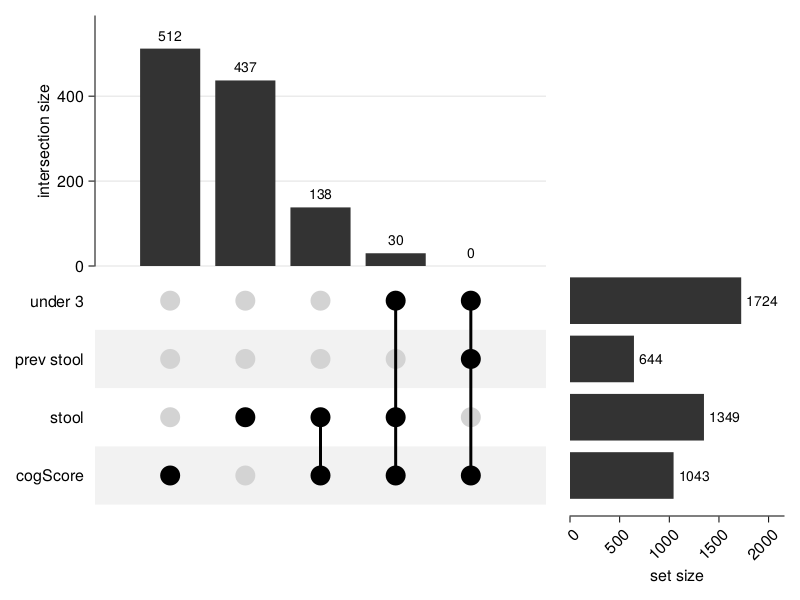
\includegraphics[width=1\linewidth]{../figures/upset_score_stool_under3.pdf}
        \end{figure}

        \column{.4\textwidth} % Right column and width
    
        \textbf{Details}
        \begin{itemize}
            \item Overlap of sample collection and cognitive score for kids under 3
            \item "Under 3" row is all timepoints, regardless of stool collection
        \end{itemize}

    \end{columns}

\end{frame}

% -----------------------------------------------------------------------------
\begin{frame}{Upset - By subject}
    \begin{columns}[c] % The "c" option specifies centered vertical alignment while the "t" option is used for top vertical alignment

        \column{.6\textwidth} % Right column and width
    
        \begin{figure}
        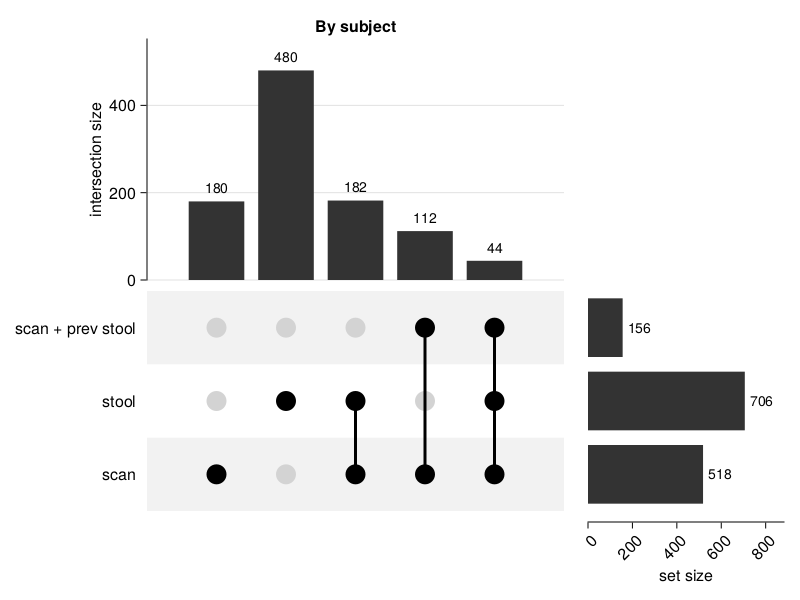
\includegraphics[width=1\linewidth]{../figures/upset_scan_stool_bysybject.pdf}
        \end{figure}

        \column{.4\textwidth} % Right column and width
    
        \textbf{Details}
        \begin{itemize}
            \item Numbers reduced to unique subjects
        \end{itemize}

    \end{columns}

\end{frame}

% -----------------------------------------------------------------------------
